\documentclass[12pt,a4paper]{scrartcl}
\usepackage[utf8]{inputenc}
\usepackage[english,russian]{babel}
\usepackage{amssymb,amsfonts}
\usepackage{amsmath,cite,enumerate}
\usepackage{float,indentfirst}
\usepackage{graphicx}
\usepackage{geometry} % Меняем поля страницы
\geometry{left=2cm}% левое поле
\geometry{right=1.5cm}% правое поле
\geometry{top=1cm}% верхнее поле
\geometry{bottom=2cm}% нижнее поле
\graphicspath{{images/}}

\begin{document}


\begin{titlepage}
  \begin{center}
    Санкт-Петербургский Политехнический Университет     Петра Великого \\
    
    Институт компьютерных наук и технологий \\
    
    Кафедра компьютерных систем и программных технологий
  \end{center}
  
  \vfill
  
  \begin{center}
  Лабораторная работа №6\\
  по теме\\
  "Цифровая модуляция"\\
\end{center}

\vfill

\newlength{\ML}
\settowidth{\ML}{«\underline{\hspace{0.7cm}}» \underline{\hspace{2cm}}}
\hfill\begin{minipage}{0.4\textwidth}
  Выполнил студент группы 33501/3\\
  \underline{\hspace{\ML}} Кисличенко Б.\,Д\\
\end{minipage}%

\bigskip

\settowidth{\ML}{«\underline{\hspace{0.7cm}}» \underline{\hspace{2cm}}}
\hfill\begin{minipage}{0.4\textwidth}
  Руководитель\\
  \underline{\hspace{\ML}} Богач Н.\,В\\
\end{minipage}%

\vfill
 
\begin{center}
  Санкт-Петербург\\
2018 
\end{center}

\end{titlepage}

\section{Цель}
\label{sec:goal}

Изучение методов модуляции цифровых сигналов.\\

\section{Постановка задачи}
\label{sec:task}

1) Получить сигналы BPSK, PSK, OQPSK, genQAM, MSK, M-FSK модуляторов.

2) Построить их сигнальные созвездия.

3) Провести сравнение изученных методов модуляции цифровых сигналов.

\clearpage
\newpage

\section{Цифровая модуляция}
\label{sec:teoriya}

Числа при передаче информации в цифровой форме с периодом Т поступают от источника информации и называются символами (symbol), а частота передачи символов – символьной скоростью (symbol rate) $f_T = 1/T$. В практике передачи данных распространена двоичная (binary) последовательность символов, где числа передаются значениями 0 и 1.


Каждому из возможных символов устанавливается определенный набор параметров несущего колебания, которые поддерживаются постоянными на интервале Т до прихода следующего символа. Это означает преобразование последовательности чисел в ступенчатый сигнал, который используется в качестве модулирующего сигнала. Соответственно, параметры несущего колебания, на которые переносится сигнал, меняются скачкообразно. Такой способ модуляции несущей обычно называется \textbf{манипуляцией} (keying).

В зависимости от изменяемых параметров манипуляцию разделяют на амплитудную, фазовую, частотную и квадратурную.

При \textbf{частотной манипуляции} (ЧМн; английский термин - frequency shift keying,\textbf{FSK}) каждому возможному значению передаваемого символа сопоставляется своя частота. В течение каждого символьного интервала передается гармоническое колебание с частотой, соответствующей текущему символу.

\textbf{MSK} (minimum shift key) - \textbf{манипуляция с минимальным сдвигом частоты.} Разность частот сигналов, соответствующих различным битам, равна половине скорости передачи информации. Манипуляция называется с минимальным сдвигом частоты, так как значение $\Delta f = \frac{1}{2T}$ является минимальной разностью частот, при котором сигналы с различными частотами, являются ортогональными. 

\textbf{MFSK} - \textbf{Многопозиционная частотная манипуляция.} Метод манипуляции, при котором N дискретных состояних входного сигнала преобразуются в набор из N фиксированных частот, передаваемых параллельно или последовательно.

\textbf{Амплитудная манипуляция} (АМн; английский термин - amplitude shift keying, \textbf{ASK}), при которой скачкообразно меняется амплитуда несущего колебания, является частным случаем квадратурной манипуляции.

\textbf{Фазовая манипуляция} (ФМн; английский термин - phase shift keying, \textbf{PSK}), при которой скачкообразно меняется фаза несущего колебания, тоже является частным случаем квадратурной манипуляции.

Фазоманипулированный сигнал имеет следующий вид:

$$s_m(t)=g(t)cos[2\pi f_c t +\phi_m (t)],$$
где g(t) определяет огибающую сигнала: $\phi_m (t)$ является модулирующим сигналом. $\phi_m (t)$ может принимать M дискретных значений. $f_c$ - частота несущей; t - время.

Если M=2, то фазовая манипуляция называется двоичной фазовой манипуляцией (\textbf{BPSK}, B-Binary — 1 бит на 1 смену фазы), если M=4 — квадратурной фазовой манипуляцией (\textbf{QPSK}, Q-Quadro — 2 бита на 1 смену фазы)

ini_phase задает начальную фазу комплексной огибающей в радианах\textbf{OQPSK} (Offset QPSK) - \textbf{Четырехфазная ФМ со сдвигом}. Позволяет избежать скачков фазы на 180° и, следовательно, глубокой модуляции огибающей. Формирование сигнала в модуляторе OQPSK происходит так же, как и в модуляторе ФМ-4, за исключением того, что манипуляционные элементы информационных последовательностей x(t) и y(t) смещены во времени на длительность одного элемента Т.

При \textbf{квадратурной манипуляции} (КАМн; английский термин - quadrature amplitude shift keying, \textbf{QASK}) каждому из возможных значений дискретного символа $C_k$ ставится в соответствие пара величин - амплитуды синфазной и квадратурной составляющих либо, что эквивалентно, амплитуда и начальная фаза несущего колебания:
$$C_k->(a_k,b_k), s(t)=a_k cos \omega_0 t+b_k sin \omega_0 t, kT<=t<(k+1)T$$
Параметры аналогового колебания, сопоставленные дискретному символу $C_k$,
удобно представлять в виде комплексного числа в алгебраической $(a_k + jb_k)$ или
экспоненциальной $(A_k exp(j \phi_k))$ форме. Совокупность этих комплексных чисел для всех возможных значений дискретного символа называется \textbf{сигнальным созвездием}.

При представлении дискретного символа комплексным числом $C_k$ сигнал с квадратурной манипуляцией можно записать следующим образом: $$s(t)=Re(C_k exp(-j \omega_0 t)), kT<=t<(k+1)T.$$ 

\clearpage
\newpage
\section{Работаем в Matlab}
\label{sec:AM}

\subsection{BPSK}
\label{sec:BPSK}
%Рисунок 1
\begin{figure}[h!]
\center{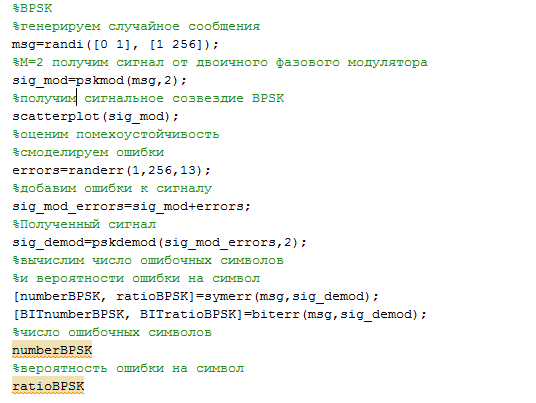
\includegraphics[width=0.9\linewidth]{bpsk_code}}
\caption{Код Matlab (BPSK)}
\end{figure}

%Рисунок 2
\begin{figure}[h!]
\center{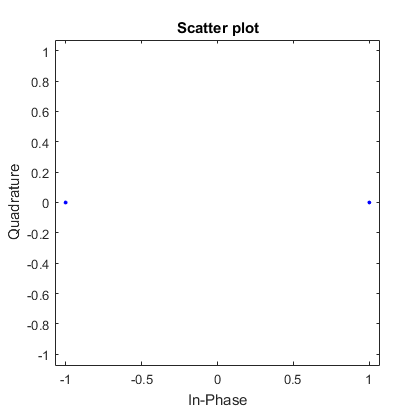
\includegraphics[width=0.5\linewidth]{BPSK}}
\caption{Сигнальное созвездие BPSK}
\end{figure}

\clearpage
\newpage

\subsection{PSK}
\label{sec:PSK}
%Рисунок 3
\begin{figure}[h!]
\center{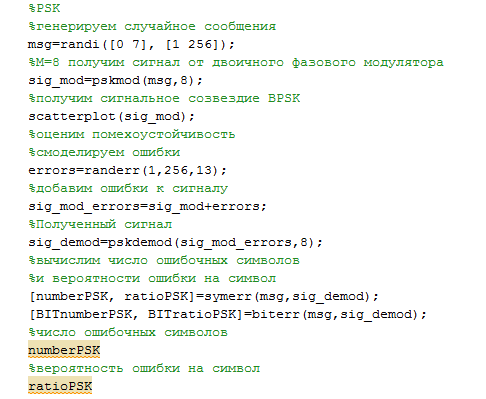
\includegraphics[width=0.9\linewidth]{PSK_code}}
\caption{Код Matlab (PSK)}
\end{figure}

%Рисунок 4
\begin{figure}[h!]
\center{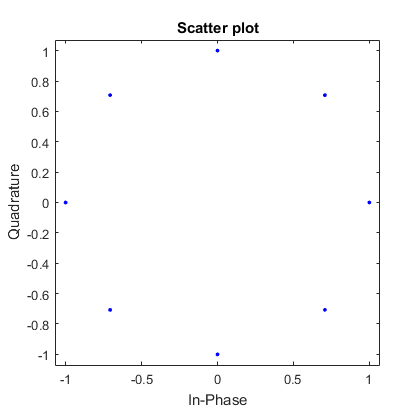
\includegraphics[width=0.5\linewidth]{PSK}}
\caption{Сигнальное созвездие PSK}
\end{figure}

\clearpage
\newpage
\subsection{OQPSK}
\label{sec:OQPSK}
%Рисунок 5
\begin{figure}[h!]
\center{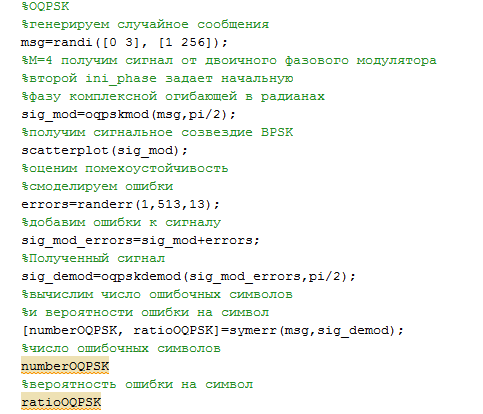
\includegraphics[width=0.9\linewidth]{OQPSK_code}}
\caption{Код Matlab (OQPSK)}
\end{figure}

%Рисунок 6
\begin{figure}[h!]
\center{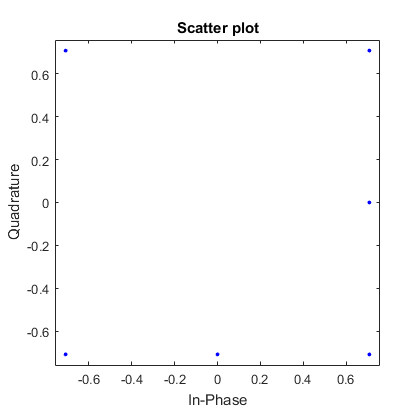
\includegraphics[width=0.5\linewidth]{OQPSK}}
\caption{Сигнальное созвездие OQPSK}
\end{figure}

\clearpage
\newpage
\subsection{genQAM}
\label{sec:genQAM}
%Рисунок 7
\begin{figure}[h!]
\center{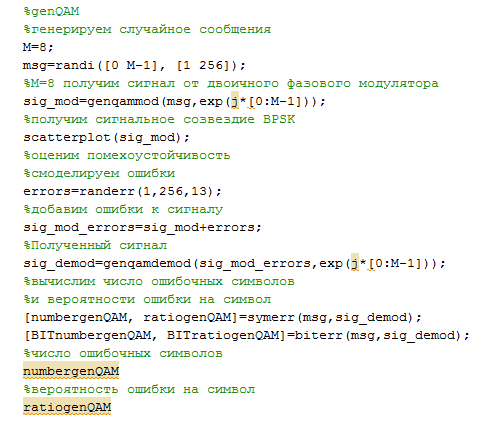
\includegraphics[width=0.8\linewidth]{genQAM_code}}
\caption{Код Matlab (genQAM)}
\end{figure}

%Рисунок 8
\begin{figure}[h!]
\center{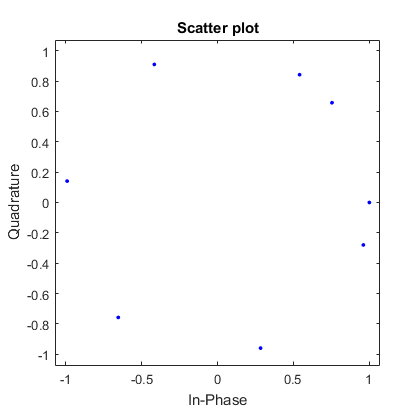
\includegraphics[width=0.5\linewidth]{genQAM}}
\caption{Сигнальное созвездие genQAM}
\end{figure}

\clearpage
\newpage
\subsection{MSK}
\label{sec:MSK}
%Рисунок 9
\begin{figure}[h!]
\center{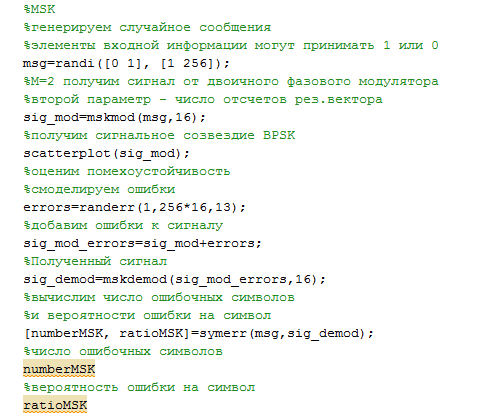
\includegraphics[width=0.9\linewidth]{MSK_code}}
\caption{Код Matlab (MSK)}
\end{figure}

%Рисунок 10
\begin{figure}[h!]
\center{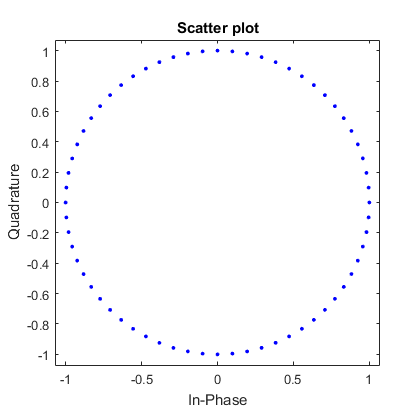
\includegraphics[width=0.5\linewidth]{MSK}}
\caption{Сигнальное созвездие MSK}
\end{figure}

\clearpage
\newpage
\subsection{FSK}
\label{sec:FSK}
%Рисунок 11
\begin{figure}[h!]
\center{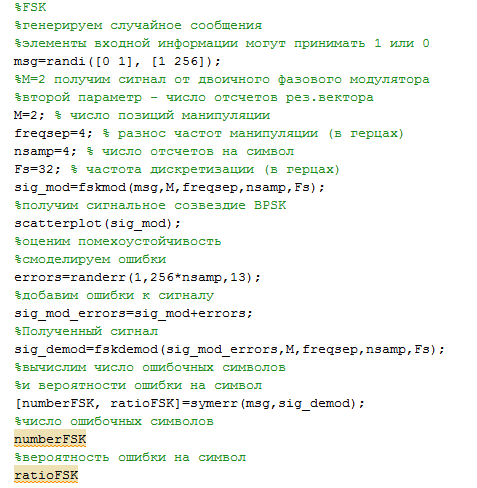
\includegraphics[width=0.7\linewidth]{FSK_code}}
\caption{Код Matlab (FSK)}
\end{figure}

%Рисунок 12
\begin{figure}[h!]
\center{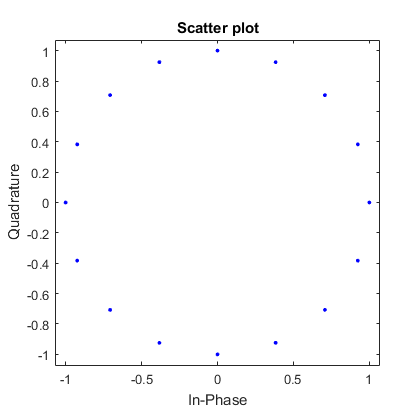
\includegraphics[width=0.5\linewidth]{FSK}}
\caption{Сигнальное созвездие FSK}
\end{figure}


\clearpage
\newpage

\section{Вывод}
\label{sec:afterWork}
За счет использования двумерного характера гармонического несущего колебания (под двумерностью здесь понимается наличие двух параметров, которые можно независимо изменять) квадратурная манипуляция обеспечивает большую помехоустойчивость (то есть меньшую вероятность ошибки), чем АМн и ФМн.

Помехоустойчивость тем выше, чем больше расстояние d между ближайшими точками созвездия на комплексной плоскости. При этом для корректности сравнения разных созвездий у них должны быть одинаковыми, помимо числа точек, среднеквадратические амплитуды:

$$\sigma=\sqrt{\frac{1}{N}\sum_{k=0}^{N-1}|C_k|^2}$$

\end{document}